\documentclass[11pt]{article}
\usepackage{amsmath,amsfonts}
\usepackage[numbers,sort&compress]{natbib}
\usepackage{times}
\usepackage[left=2.54cm,top=2.54cm,right=2.54cm,bottom=2.54cm,bindingoffset=0.0cm]{geometry}
\usepackage{setspace}
\usepackage{enumerate}
\usepackage{enumitem}
\usepackage{wrapfig}
\setcounter{secnumdepth}{0}
\usepackage{fullpage}
\usepackage{titlesec}
\titleformat{\section}{\large\bfseries}{\thesection}{1em}{}
\titleformat{\subsection}{\bfseries}{\thesubsection}{1em}{}
\usepackage{parskip} % skip paragraph indentations
\usepackage{lipsum}
\usepackage{hyperref}
\usepackage{graphicx}
\usepackage{amssymb}
\usepackage[x11names]{xcolor}
\usepackage{hyperref}
\usepackage{enumitem}
\usepackage{booktabs}
\usepackage{amsmath}
\usepackage{amssymb}
\usepackage{mathrsfs}
\usepackage{caption} \captionsetup[table]{singlelinecheck=false} %makes table captions left-justified
\usepackage{framed} % to add frames around comments
%\hypersetup{backref,colorlinks=false,
%    urlbordercolor=LightSkyBlue4,          % color of internal links
%    citebordercolor=SpringGreen4,        % color of links to bibliography
%    filebordercolor=magenta,      % color of file links
%    linkbordercolor=Red3, pdfborderstyle={/S/U/W 1.5}}
\newcommand{\Prob}[1]{\Pr{\left( #1 \right)}}
\newcommand{\q}[1]{``#1''} % easier way to get double quotes
\newcommand{\argmin}{\text{argmin}}
\usepackage{authblk} % for title page
\renewcommand\Affilfont{\fontsize{10}{10.8}\itshape}
\renewcommand\familydefault{\sfdefault} 
\usepackage{datetime2}
%\renewcommand{\dateseparator}{-}
\usepackage{atbegshi}% http://ctan.org/pkg/atbegshi -- removes blank page at start of doc
\AtBeginDocument{\AtBeginShipoutNext{\AtBeginShipoutDiscard}}
\setcounter{page}{0}
\begin{document}
\noindent
\title{Draft: Learned badges vs. Social recognition} 
%The evolution of rank signaling?

\author[1]{Eleanor Brush}
\affil[1]{University of Maryland; email: xxxxx}
\author[2,3]{Elizabeth A. Hobson}
\affil[2]{Santa Fe Institute, 1399 Hyde Park Road, Santa Fe, NM 87501 USA}
\affil[3]{National Institute for Mathematical and Biological Synthesis, University of Tennessee, Knoxville, TN, USA; email: ehobson@santafe.edu}
%\date{} 
\maketitle

%%%%%%%%%%%%%%%%%%%%%%%
\section*{Overview of previous research, outstanding questions, goals} 
%%%%%%%%%%%%%%%%%%%%%%%

Species have different ways of assessing the quality of others. Quality here is used broadly, and can indicate an individual's body condition or immune status, overall reproductive potential, or fitness. Individuals can gain long-term benefits from assessing each others' quality. In the context of conflicts when individuals differ in fighting ability, resource-holding potential, or dominance rank, it may be beneficial for individuals to be able to identify and order individuals by quality. 

% summary of previous research
...Lots of investigation into evolution of 'honest' signaling...  


% summary of our focus for the modeling work (learned badge vs learned recognition) 

Species have different ways of assessing the quality of others. Here, we focus on one type of signal -- the badge of status -- and compare it to a system based on individual recognition. A badge is an arbitrary signal, not directly indicative of fighting ability, where the intensity of the signal correlates with the underlying quality of the individual (here, rank/power) (CITE). Another quality assessment system is a combination recognition/relationship method, where individuals that are able to recognize individuals track their actions and event outcomes to infer quality in the absence of a cue or badge of status (CITE). In both cases, individuals must learn about their opponents in order to assess their quality.

At the two extremes, individuals in a pure badge quality signal system would be completely unable to recognize individuals, and would treat all individuals with similar badge intensities as equivalent; individuals in a pure recognition/relationships based quality system would be completely reliant on remembering an individual's actions, and have no other cues to infer that individual's quality or rank. Binning individuals with similar badge intensities into the same category effectively decreases the functional group size to the number of bins, but also increases noise about quality of each individual. An individual recognition-based system is one in which the number of bins equals the number of individuals in the group.  

\subsection*{Justification and Goals}

[this is a bit rough] Many factors likely affect the accuracy and speed of quality assessment in these two systems. Recent work (\cite{sheehan2016evotradeoff}) provides several predictions but focused on predicting differences in signaling systems comparing an innate quality signal to a social recognition system across different species, not within species (\cite{sheehan2016response}). Here, we use a somewhat different approach: we are interested in two hypothetical systems, where individuals learn to assess quality to others in different ways. 

Our goal is to better understand the conditions under which a badge signal or individual recognition would be favored. We simulated quality assessment through fights among individuals. Each time individuals fight, they are able to assess each other's quality and update their previous opinion about quality. We use two quality assessment methods: (1) Badge signal systems: individuals group others into quality categories based on the intensity of badge signals and (2) Recognition systems: individuals use individual recognition to remember the outcome of events with particular individuals to estimate quality. 

%%%%%%%%%%%%%%%%%%%%%%%
\section*{Methods} 
%%%%%%%%%%%%%%%%%%%%%%%
%
\subsection*{Model}
%
Animals in a social group can benefit from knowing about their peers. For example, knowing which individuals are strong and weak can help an animal decide with whom to fight. Knowing which individuals are likely to have viable and healthy offspring can help females choose a male with which to mate. In our model, each animal has an inherent \q{quality} value, $q_i$, that the other animals try to assess. An animal's quality is only revealed when it engages in a fight. Each animal also displays a \q{signal}, $s_i$, which is always visible. We define the parameter $\rho$ as the correlation between the signals, $\{s_i\}$, and the quality values, $\{q_i\}$. (A list of the variables used in the text is provided in Table \ref{tab:vars}.) To simulate a particular social group, we draw $N$ values $\{q_1,\dots,q_N\}$ from a normal distribution with mean $0$ and standard deviation $\sigma_\text{q}$. We then generate $N$ signal values such that $\min_i{s_i}\approx -1$, $\max_i{s_i}\approx 1$, and the correlation between $\{q_i\}$ and $\{s_i\}$ is precisely $\rho$.
  
At first, the group consists entirely of naive animals, none of whom have any knowledge of each other. The animals learn about the quality of each of the other animals based on fights in which pairs of animals engage. At first, animals can only learn directly from their own experiences in fights. Below, we consider the possibility of observational learning, where animals can additionally learn from watching the outcomes of fights in which they are not involved.  

We consider two types of learning: individual and categorical learning. An individual learner can recognize each of the other individuals in its group and successively refine its estimate of each of their quality values. A categorical learner only recognizes animals based on the signals they display. A categorical learner has a perceptive threshold, such that if two animals have sufficiently similar signals, it will perceive them to be the same. Every time it encounters an animal it perceives to be in a given category, it updates its estimate of the quality of animals in that category. For example, if an animal has very poor perceptive abilities, it might only be able to identify animals with small, medium, and large signals, and the best it can do is to try to learn about animals in each of those categories. 

A categorical learner forms these categories before any fights occur. Specifically, two animals are perceived to be the same if the difference in their signals is less than $\delta$, $|s_j-s_k|<\delta$. A focal animal picks one animal, $j$ at random. All animals whose signals are within $\delta$ of $s_j$ are put in the same category. Then the focal animal picks an uncategorized animal at random, $k$, forming a second category of all uncategorized animals whose signals are within $\delta$ of $s_k$. It proceeds this way until every animal in the group has been assigned a category.  Figure \ref{cats_ex} shows one example of this process. Depending on how each animal forms its categories, different animals will categorize the group differently and may perceive different numbers of categories. Each individual $i$ will identify a category $k$ by the median of the signal being displayed by individuals in that category, $\bar{s}_{ik}$. The average number of categories  animals perceive depends on the size of the group and the perceptive ability, $\delta$ (Supp Figure XX). 

At each time step, the animals forget their opinions of individuals or categories they encountered longer than a time window, $w$ steps, ago. An individual learner will maintain its opinions of animals they encountered fewer than $w$ time steps ago. A categorical learner re-categorizes the rest of the group at each time step. Specifically, animal $i$ puts animal $j$ in category $k$ with probability 
\begin{equation*}
\frac{\exp(-r_\text{cat}|s_j-\bar{s}_{ik}|)}{\sum_\ell\exp(-r_\text{cat}|s_j-\bar{s}_{il}|)},
\end{equation*}
where $r_\text{cat}$ describes the reliability of the categories over time: if $r_\text{cat}=\infty$, $i$ categorizes the group the same way at every time step and as $r_\text{cat}$ the probability of re-categorizing animals increases. If $i$ remembers its opinion of category $k$, it assigns that opinion to all individuals it now perceives as being in category $k$. 
Next, we randomly choose two individuals to \q{fight}. 
%The animal with higher quality is more likely to win. Specifically, the probability of $i$ winning in a fight against $j$ is 
%\begin{equation*}
%\frac{\exp\big(b(q_i-q_j)\big)}{\exp\big(b(q_i-q_j)\big)+1},
%\end{equation*}
%where $b$ represents the bias in the fight: if $b=0$, then both animals are equally likely to win, regardless of their qualities, and if $b$ is large, the stronger animals wins with near certainty. 
An individual learner correctly identifies its opponent with probability $r_\text{ind}$. With probability $1-r_\text{ind}$ it misidentifies its opponent as another randomly chosen member of the group.  A categorical learner perceives the category of its opponent with the probabilities just described. Each animal in the fight updates its opinion of the individual or category it perceives in its opponent. If $a_{ij}(t-1)$ is $i$'s opinion of $j$ at time $t-1$, after fighting, 
\begin{equation*}
a_{ij}(t)=(1-\ell)a_{ij}(t-1)+\ell q_j+\xi,
\end{equation*}
where $\ell$ is a parameter describing how much $i$ changes its opinion based on its observation and $\xi$ is drawn from a normal distribution with mean $0$ and standard deviation $\sigma_\xi$. If $i$ and $j$ have not fought before or $i$ has forgotten its opinion of $j$, then after fighting 
\begin{equation*}
a_{ij}(t+1)=(1-r)b_{i}(t)+rq_j+\xi,
\end{equation*}
where $b_i(t)$ is a baseline opinion of any animal it encounters. Specifically, $b_i(t)$ is drawn from a normal distribution with mean equal to the average quality of the group and standard deviation $\sigma_\text{b}$. 

In a given simulation, we keep track of each animal's opinion of every other for $T$ fights. This allows us to calculate the error of each animal's opinion of every other at each point in time, $|a_{ij}(t)-q_j|$. To measure each animal's learning ability, we average its error over the rest of the group. 
\begin{equation*}
\epsilon_i(t) = \frac{1}{|\mathscr{O}_i(t)|}\sum_{j\in \mathscr{O}_i(t)}|a_{ij}(t)-q_j|,
\end{equation*}
where $\mathscr{O}_i(t)$ is the set of animals about whom $i$ has an opinion at time $t$.
We also calculate an animal's learning time about another individual as the first point in time at which its error about that individual drops below a threshold $\bar{\epsilon}$. We then average its learning time about each of the other animals in the group:
\begin{equation*}
\tau_{i} = \frac{1}{|\mathscr{O}_i|} \sum_{j\in\mathscr{O}_i} \min_{t=1,\dots,T}\{t: \epsilon_{ij}(t)\leq\bar{\epsilon}\}.
\end{equation*}
%
\subsection*{Parameter space}
%
We investigated how varying several parameters affected the learning curves, learning accuracy, and learning time. We varied group size ($N=\{25, 50, 75, 100\}$), the correlation between the signal and underlying quality of individuals ($\rho=\{0.5,0.9\}$), the memory capabilities of agents ($w=\{200,1000,\infty\}$), and the total number of fights. For the badge signal system, we also specify the perceptive threshold that individuals use to categorize individuals by signal ($\delta=\{0,0.1,0.2,\dots,1.5\}$). For the individual learning system, we set $r_\text{ind}=1$, and for the categorical learning system, we set $r_\text{cat}=\infty$. For both types of learning, we set $\bar{\epsilon}=0.2$, $\ell=0.2$, $\sigma_\text{b}=0.2$, $\sigma_\text{q}=0.5$, $\sigma_\xi=0.01$.

%
\subsection*{Variables}
%
\begin {table}[h]
\caption {Description of variables} \label{tab:vars} 
\begin{tabular}{cl}
\toprule
 Variables & Description of variables \\
\midrule 
$\delta$ & perceptive threshold \\
$\epsilon_i$ & learning accuracy of individual $i$ (averaged across all $j$ individuals) \\
$\bar{\epsilon}$ & threshold error for defining learning time \\
$\ell$ & learning rate \\
$N$ & number of individuals \\ 
 $q_i$ & quality of individual i \\ 
$\rho$ & correlation between quality and signal \\
$s_i$ & signal of quality / badge of status of individual $i$ \\ 
$w$ & memory window \\
$\sigma_\text{b}$ & standard deviation of baseline opinion \\
$\sigma_\text{q}$ & standard deviation of quality values \\
$\sigma_\xi$ & standard deviation of noise in opinion updating \\
$T$ & total number of fights \\
\bottomrule
\end{tabular}
\end {table}
%
\subsection*{Defining categories}
%
\textbf{Email text: }I noticed at the end of the day yesterday that since I've changed how the categories are created, for a given perception window, there are fewer categories when signal and quality are poorly correlated, i.e. holding perception window constant but varying correlation changes the number of categories the animals perceive. I'll explain why this happened below if you care, but I've rewritten the code so that varying correlation doesn't affect the number of categories being perceived. It's better because we can only identify the effects of the signal-quality correlation and the perception abilities if they're independent parameters. Since all the lines in the summary plots hold correlation constant, so it shouldn't change any results. 

The issue was in how I generated signal values: First, I draw quality values from a normal distribution. Then, I draw signal values from a normal distribution and rotate them so that the signal values have the desired correlation with the quality values. The way I was rotating kind of squashed the signal values together when correlation was low and spread them out when correlation was high. This didn't matter when we were using number of categories as a parameter because we'd just divvy up the group into that many categories. However, using a perception window, the more similar the animals are, the fewer categories they get binned into, so low correlation meant few categories. I've rewritten how the signal values are generated so that there is more or less the same amount of variation regardless of the quality-signal correlation.

\textbf{Email text: }I reran all the simulations with a new-and-improved way of fixing the correlation between quality and signal and generated new figures. They are, with the exception of running slightly fewer parameters for the sake of time, pretty much identical to the old. I left the old ones in the Dropbox folder just so you could compare and they have "old" at the end of the filename. Figures without "old" are good to go.

"Categories.pdf" is an example of how 25 animals might be categorized when the perception window is 0.3.

"numberofcategories.pdf" shows how the number of categories the group gets divided into depends on the perception window and the group size, in case you'd like to see.
%
\subsection*{learning times}
%
\textbf{Email text:} Re: learning time: Within one simulation of one group, I calculate an animal's learning time as the average number of fights it takes to decrease the error in its assessment about each other animal below a threshold, right now, 0.2. For each combination of parameters, I average this learning time across all individuals and all 25 simulations. This is indeed a little different than the first version of the model, where I calculated learning time as the number of fights it takes for error to get within a threshold of its final error, which doesn't make as much sense.

\textbf{Email text: }I got to wondering why learning time is much higher for individual learning when the perception window is 0, since both individual and categorical learners can identify all individuals in the group. I meant to have the probability of confusion be 0 for both types of learning, but I realized that the parameter I've been using  for categorical learning actually allowed for a small probability of two individuals being put in the same category. This means that, if an animal encounters and learns about another animal, there is a small probability that it updates its opinion about other animals that are sufficiently similar. This non-zero probability of confusion actually allows categorical learners to learn more quickly. That to me is a potentially interesting result. BUT for the moment, I'm rerunning simulations where both types of learning have 0 probability of confusion. When I get the chance, I'm planning on a more systematic sweep of the confusion probabilities to see what their effects are. If you use the current figures and someone asks why individual learning takes longer, that's why, and I'll get new figures to you as soon as I can.

\textbf{Email text:} Within one simulation of one group, each animal has an assessment about every other animal at each point in time (it may be NA). Its error about each other animal at each point in time is the absolute difference between that assessment and each other animal's quality (if the assessment is NA, the error is NA). An animal's learning time about each other animal is the number of fights before its error drops below 0.2. Error fluctuates because the animals forget and because there's some noise in every assessment they make. Even though i's error about j dropped below 0.2, it might go back up again. And just because i's error about j is below 0.2, its error about other animals might still be high. So its average error about every other animal might be above the threshold, even while its error about some or all of the other animals has already dropped below the threshold. To generate the learning curves, I take the average of this average error across all individuals and all simulations. So this average can be above the threshold, even while the average learning time is finite. I hope that makes sense. Like I said, a figure illustrating this counterintuitive calculation is on the way. 

\textbf{Email text: } See figure~\ref{learnT.ex}. The parameters are group size = 10, quality to signal correlation = 0.7, perception window = 0.5, memory window = Inf. I ran one simulation of such a group. Then I calculated the error in one animal's assessment of each other animal. There is a squiggly colored line for each of these errors over time. The squiggly black line is the average of these. The horizontal black line is the error threshold. The vertical colored lines are the "learning times" for each animal: the time when the focal animal's error about the other drops below the threshold. The vertical black line is the average of the learning times. The average error remains above the threshold, even though the animal's error about some of the other animals drops below the threshold. I tried to explain this in an earlier email, but it helps me to visualize it, hence the figure.

%%%%%%%%%%%% explanation figures

\begin{figure}[h]
\caption{\sffamily\small\textbf{Categories.}
     xxxxxxx.}
\label{cats_ex}
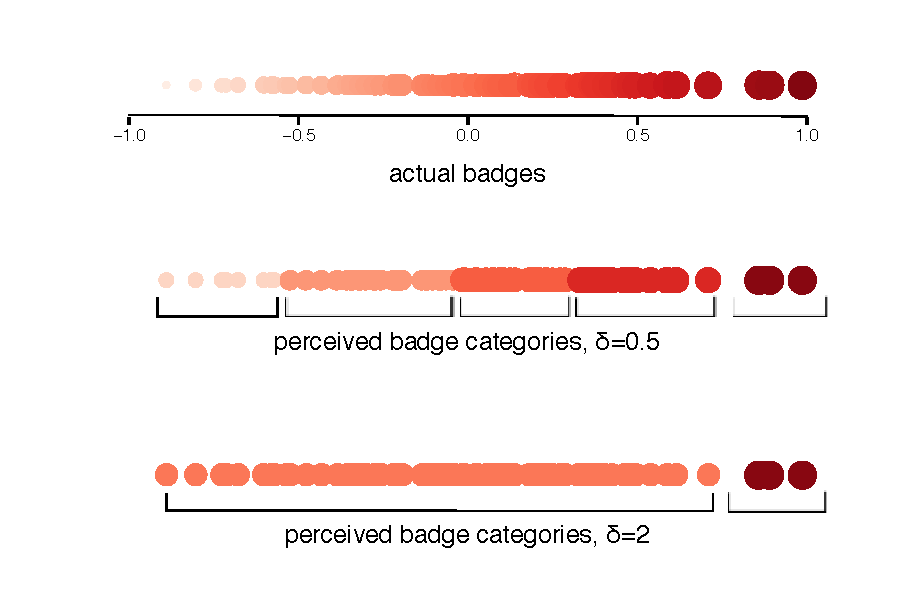
\includegraphics[width=.8\textwidth]{figures/categories.pdf}
\end{figure}

\begin{figure}[h]
\caption{\sffamily\small\textbf{Learning time example.}
     xxx.}
\label{learnT.ex}
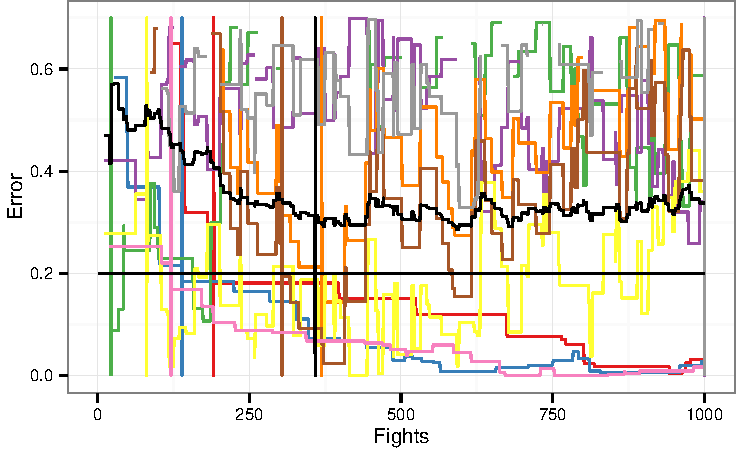
\includegraphics[width=.8\textwidth]{figures/learning_time_example.pdf}
\end{figure}
%%%%%%%%%%%%%%%%%%%%%%%%%%%

%%%%%%%%%%%%%%%%%%%%
\section*{Results}
%%%%%%%%%%%%%%%%%%%%
%
\subsection*{General results}
%
\textbf{Email text: }Red is always categorical learning. Blue is always individual learning. The average-error figures show the average (saturated line) plus or minus the standard deviation (shaded area) across all members of a group across all 25 random initial conditions. The title of each panel gives the group size (N), number of categories (number sign), window size (wind), and correlation between quality and signal (corr). All the parameters I've looked at have the expected effect, e.g. increasing group size makes individual learning more error prone. The effect-of-categor-num figure shows how the average error of categorical learning depends on the number of categories being used, for the parameters given in the title. There's a surprising shape here: the lowest error happens at an intermediate number of categories. I'm not sure why this is happening yet, but it's interesting I think. Finally, the learning-times figures give the frequencies across all individuals and all initial conditions of how long it takes the animal to get its error sufficiently close to its error after 10000 fights. Here, too, all of the parameters I've looked at have expected effects, e.g. increasing group size increases the learning time.

%
\subsection*{How do category bin sizes affect error and learning time?}
%
\subsection*{How does group size affect error and learning time?}
%
\subsection*{How does memory affect error and learning time?}
%

\begin{figure}[ht]
\caption{\sffamily\small\textbf{Learning curves.}
     Cherry-picked parameter combinations to illustrate how learning curves change under different conditions (summarized below).}
\label{learning_curves}
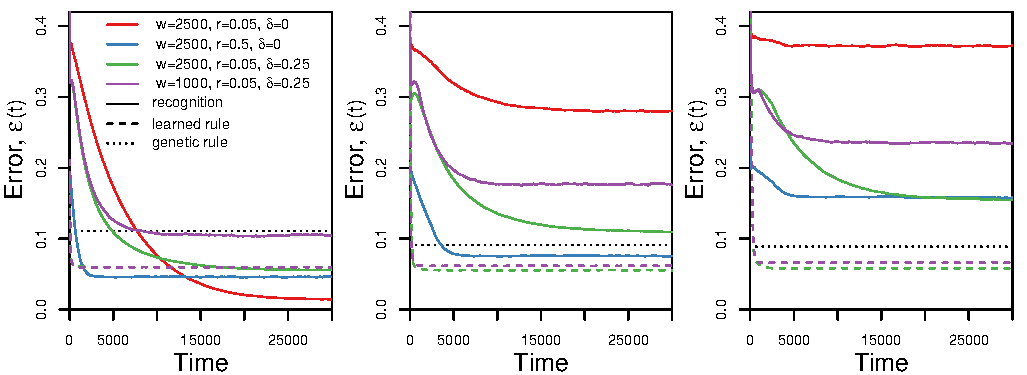
\includegraphics[width=.95\textwidth]{figures/learning_curves.pdf}
\end{figure}

\begin{figure}
\caption{\sffamily\small\textbf{Summary error by group size.}
    xxxxxxx (individualized levels shown for reference).}
\label{summary_error_groupsize}
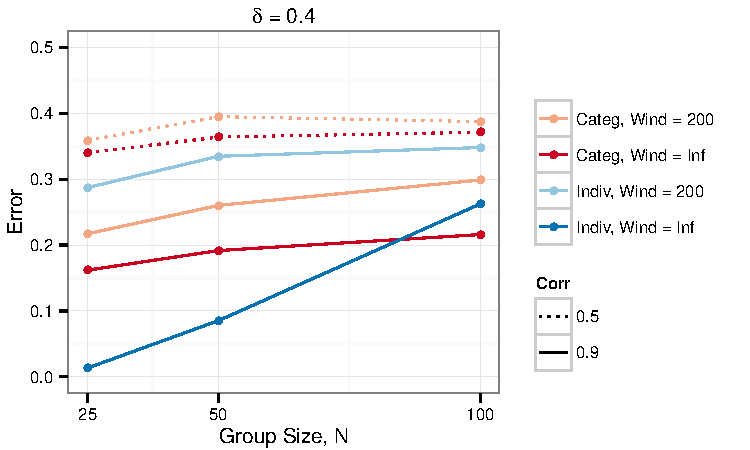
\includegraphics[width=.8\textwidth]{figures/summary_error_groupsize.pdf}
\end{figure}

\begin{figure}
\caption{\sffamily\small\textbf{Summary error by perception window.}
    xxxxxxx (individualized levels shown for reference).}
\label{summary_error}
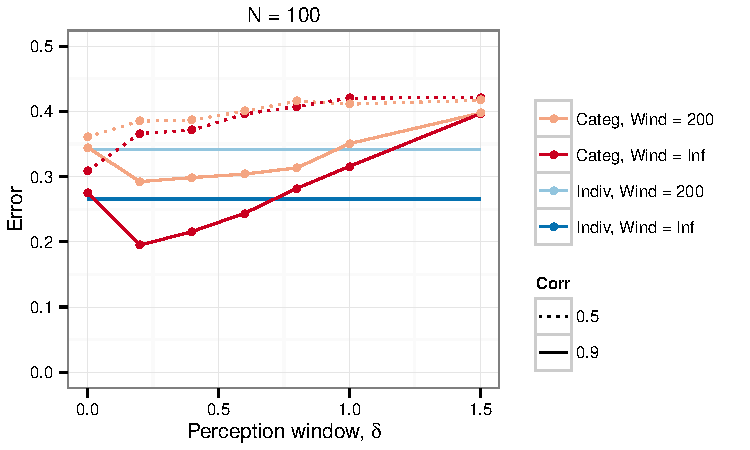
\includegraphics[width=.8\textwidth]{figures/summary_error_percwindow.pdf}
\end{figure}

\begin{figure}
\caption{\sffamily\small\textbf{Summary time by group size.}
     xxxxxxx (individualized levels shown for reference).}
\label{summary_time_groupsize}
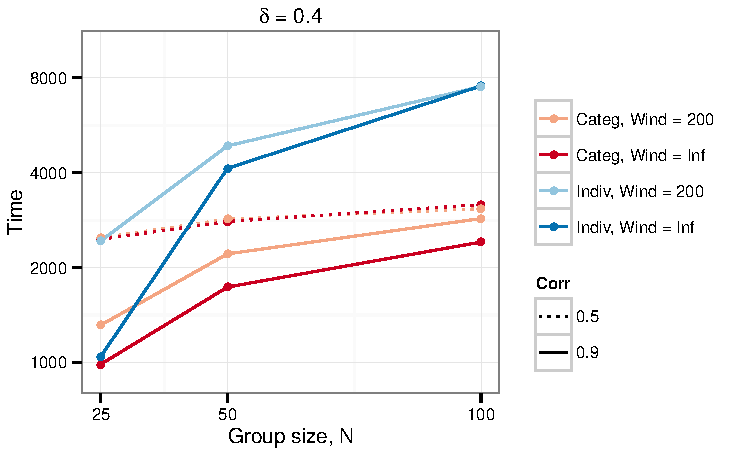
\includegraphics[width=.8\textwidth]{figures/summary_time_groupsize.pdf}
\end{figure}

\begin{figure}
\caption{\sffamily\small\textbf{Summary time by perception window.}
     xxxxxxx (individualized levels shown for reference).}
\label{summary_time_percwindow}
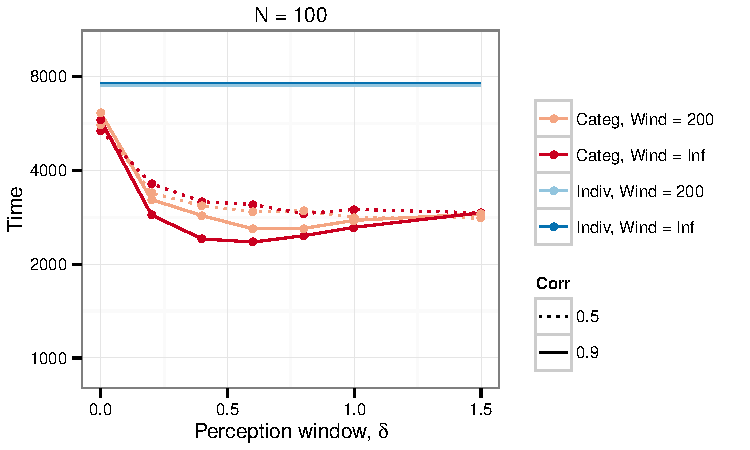
\includegraphics[width=.8\textwidth]{figures/summary_time_percwindow.pdf}
\end{figure}

%%%%%%%%%%%%%%%%%
\section*{Discussion}
%%%%%%%%%%%%%%%%%




\newpage
\bibliography{BIB_badgeVSrecog,TODO_newrefs}
\bibliographystyle{apa}

\end{document}

% CUT TEXT

% summary data quantified
We then use the simulated interaction datasets to quantify: 
\begin{enumerate}
  \item Learning curves: each individual's opinion error across the series of fights 
  \item Learning accuracy: amount of error in final opinions about quality (summarize histograms of learning error)
  \item Learning time: amount of fights (time) for opinion to achieve maximum potential accuracy (opinion at end of all fights)  
\end{enumerate}